\chapter{Data and simulated samples}\label{chap:datamc}

\section{Data}\label{sec:datamc:data}
The analysis presented in this thesis is performed on \emph{\protonproton} collision data collected by ATLAS and delivered by the LHC Run-2, between 2015 and 2018, corresponding to a total integrated luminosity of \SI{139}{\femto\barn^{-1}}. The breakdown of the luminosity collected in each year by ATLAS available for physics analysis is outlined in \cref{tab:data:lumi}. The luminosity uncertainty is determined from calibration of the luminosity scale using the Van Der Meer scans described in \cref{sec:lumi}. 
\begin{table}[h]
    \centering
    \begin{tabular}{l|c}
        Year & luminosity [\SI{}{\femto\barn^{-1}}] \\
        \hline
        2015 & 3.2 \\
        2016 & 33.0 \\
        2017 & 44.3 \\
        2018 & 59.9 \\
        \hline 
        \hline
        Total & 139 $\pm$ 1.7\% \\
	\end{tabular}
    \caption[Summary of the luminosities of datasets taken between 2015 and 2018]{Summary of the luminosities of datasets taken between 2015 and 2018~\cite{ATLAS:lumiPlots}.}
    \label{tab:data:lumi}
  \end{table}

~\cref{fig:yields2015,fig:yields2016,fig:yields2017,fig:yields2018} show the data yeilds (events per [\SI{}{\pico\barn^{-1}}) after applying the analysis selection for different data taking periods during the runs between 2015 to 2018. 

\begin{figure}[ht]
\centering
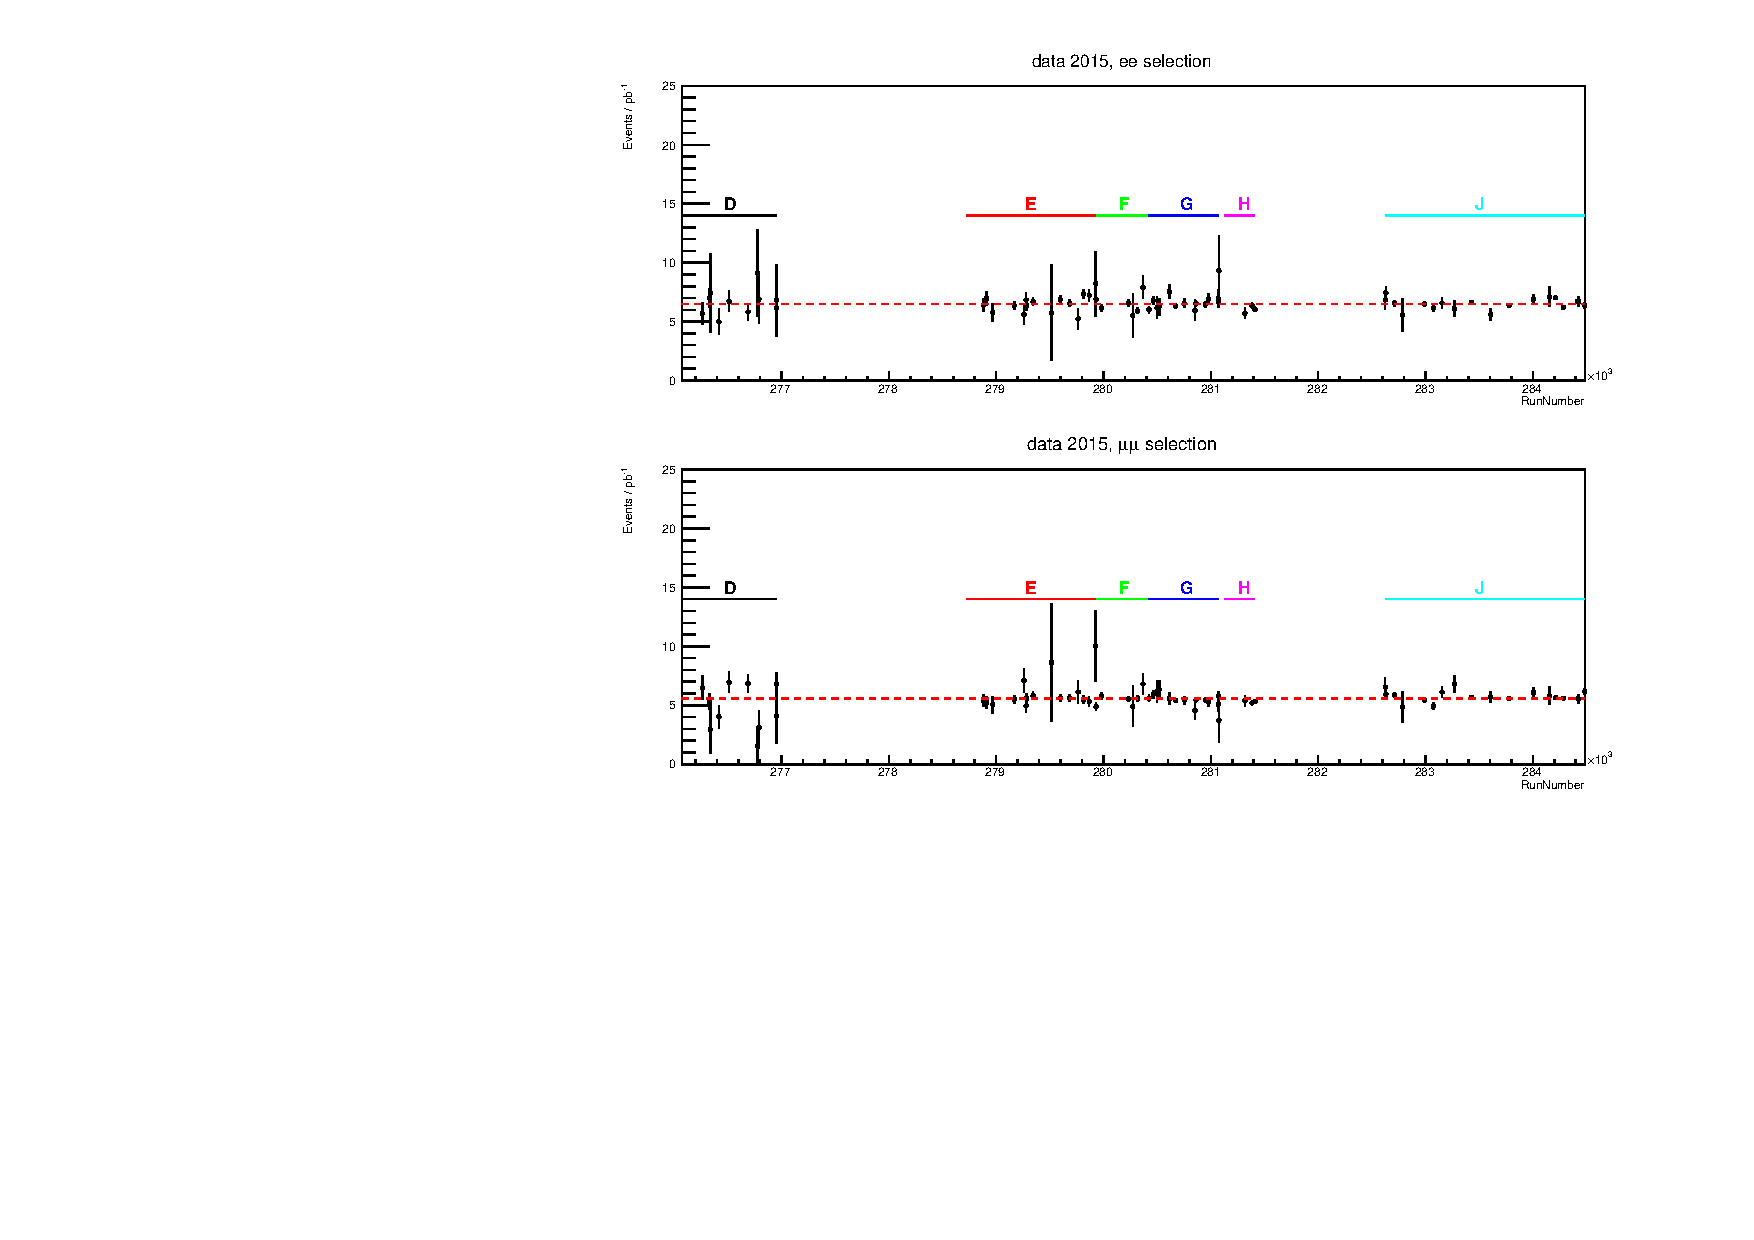
\includegraphics[width=\textwidth]{figures/analysis/datamc/Yields/compare_data_yields2015.pdf}
\caption{Data yields for the 2015 run period for the inclusive $ee$ (above) and $\mu\mu$ (below) selections. Each letter on the legend correspond to the different data taking periods within a year~\cite{Aad:2019fac}.}
\label{fig:yields2015}
\end{figure}

\begin{figure}[ht]
\centering
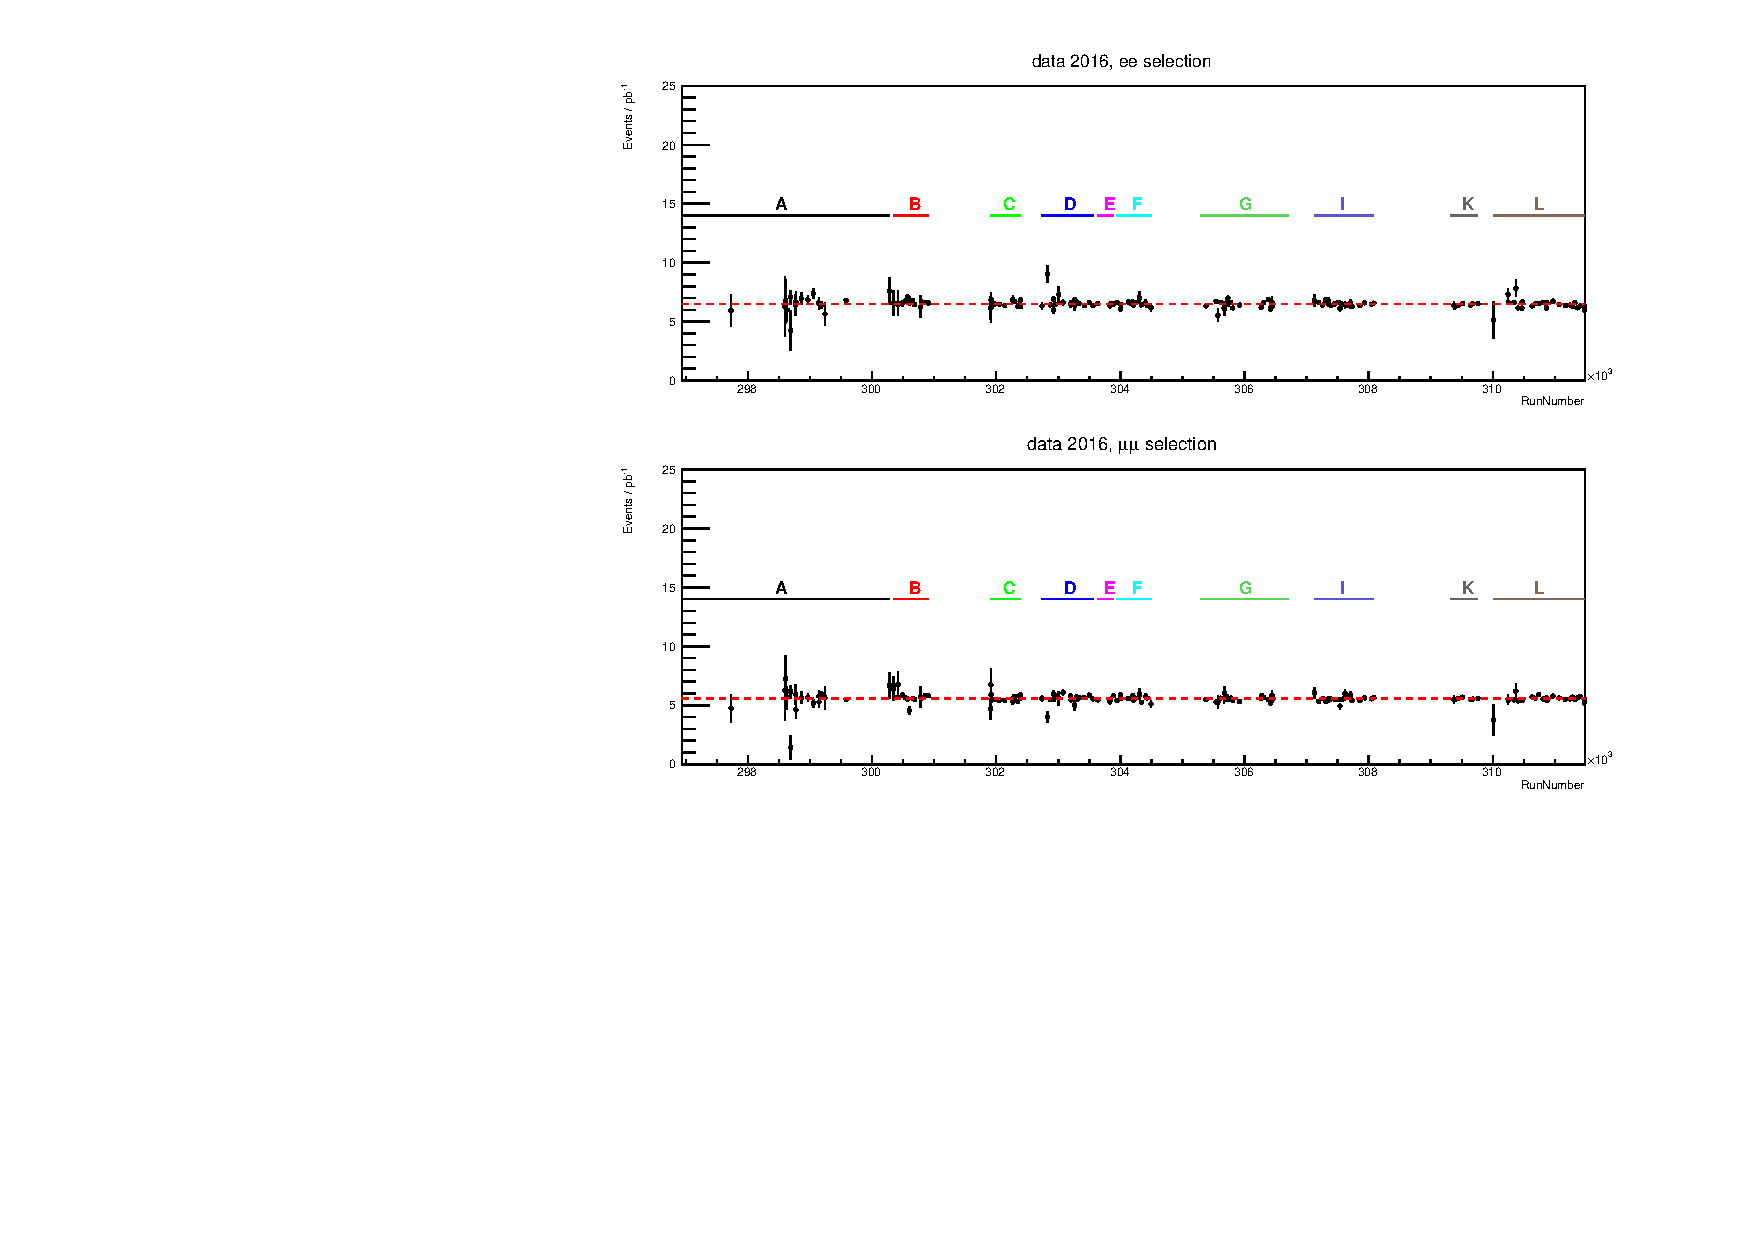
\includegraphics[width=\textwidth]{figures/analysis/datamc/Yields/compare_data_yields2016.pdf}
\caption{Data yields for the 2016 run period for the inclusive $ee$ (above) and $\mu\mu$ (below) selections. Each letter on the legend correspond to the different data taking periods within a year~\cite{Aad:2019fac}.}
\label{fig:yields2016}
\end{figure}

\begin{figure}[ht]
\centering
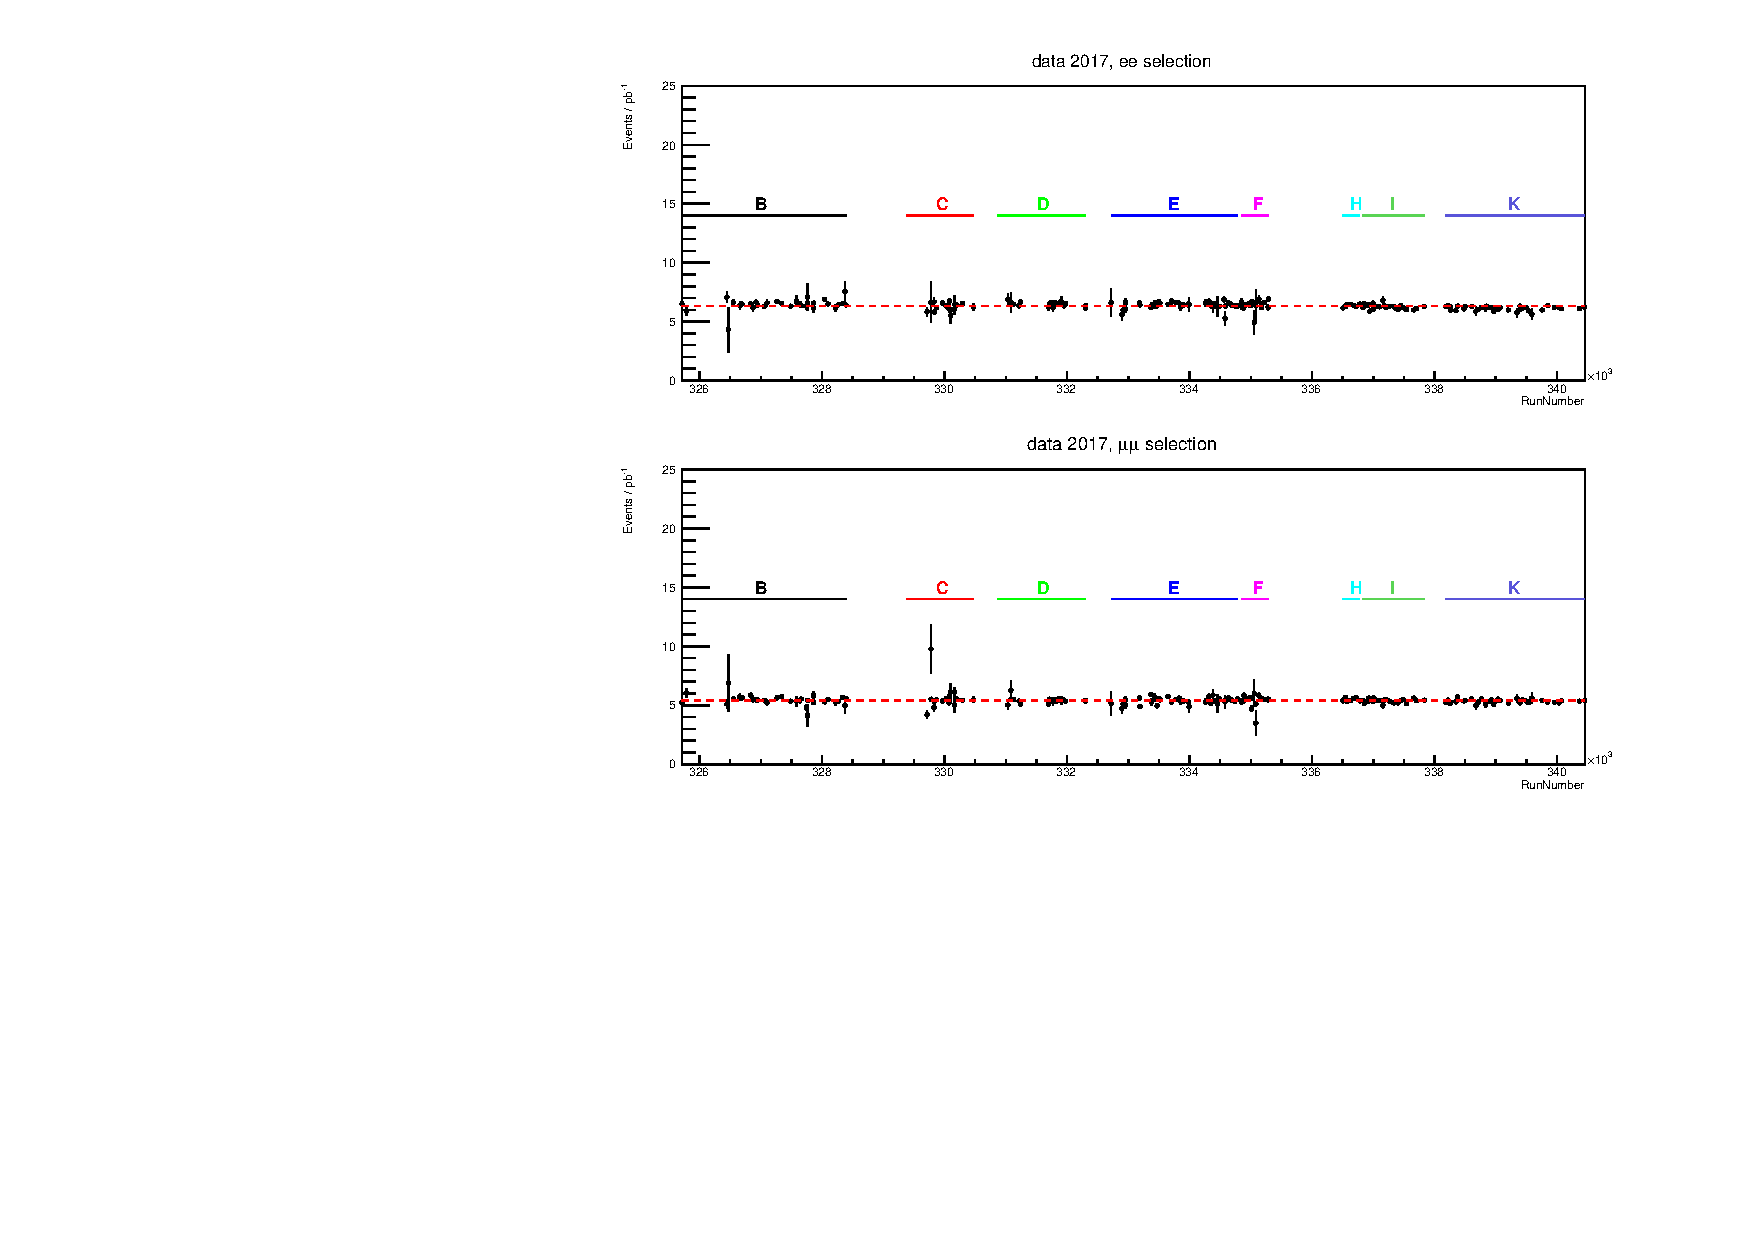
\includegraphics[width=\textwidth]{figures/analysis/datamc/Yields/compare_data_yields2017.pdf}
\caption{Data yields for the 2017 run period for the inclusive $ee$ (above) and $\mu\mu$ (below) selections. Each letter on the legend correspond to the different data taking periods within a year~\cite{Aad:2019fac}.}
\label{fig:yields2017}
\end{figure}

\begin{figure}[ht]
\centering
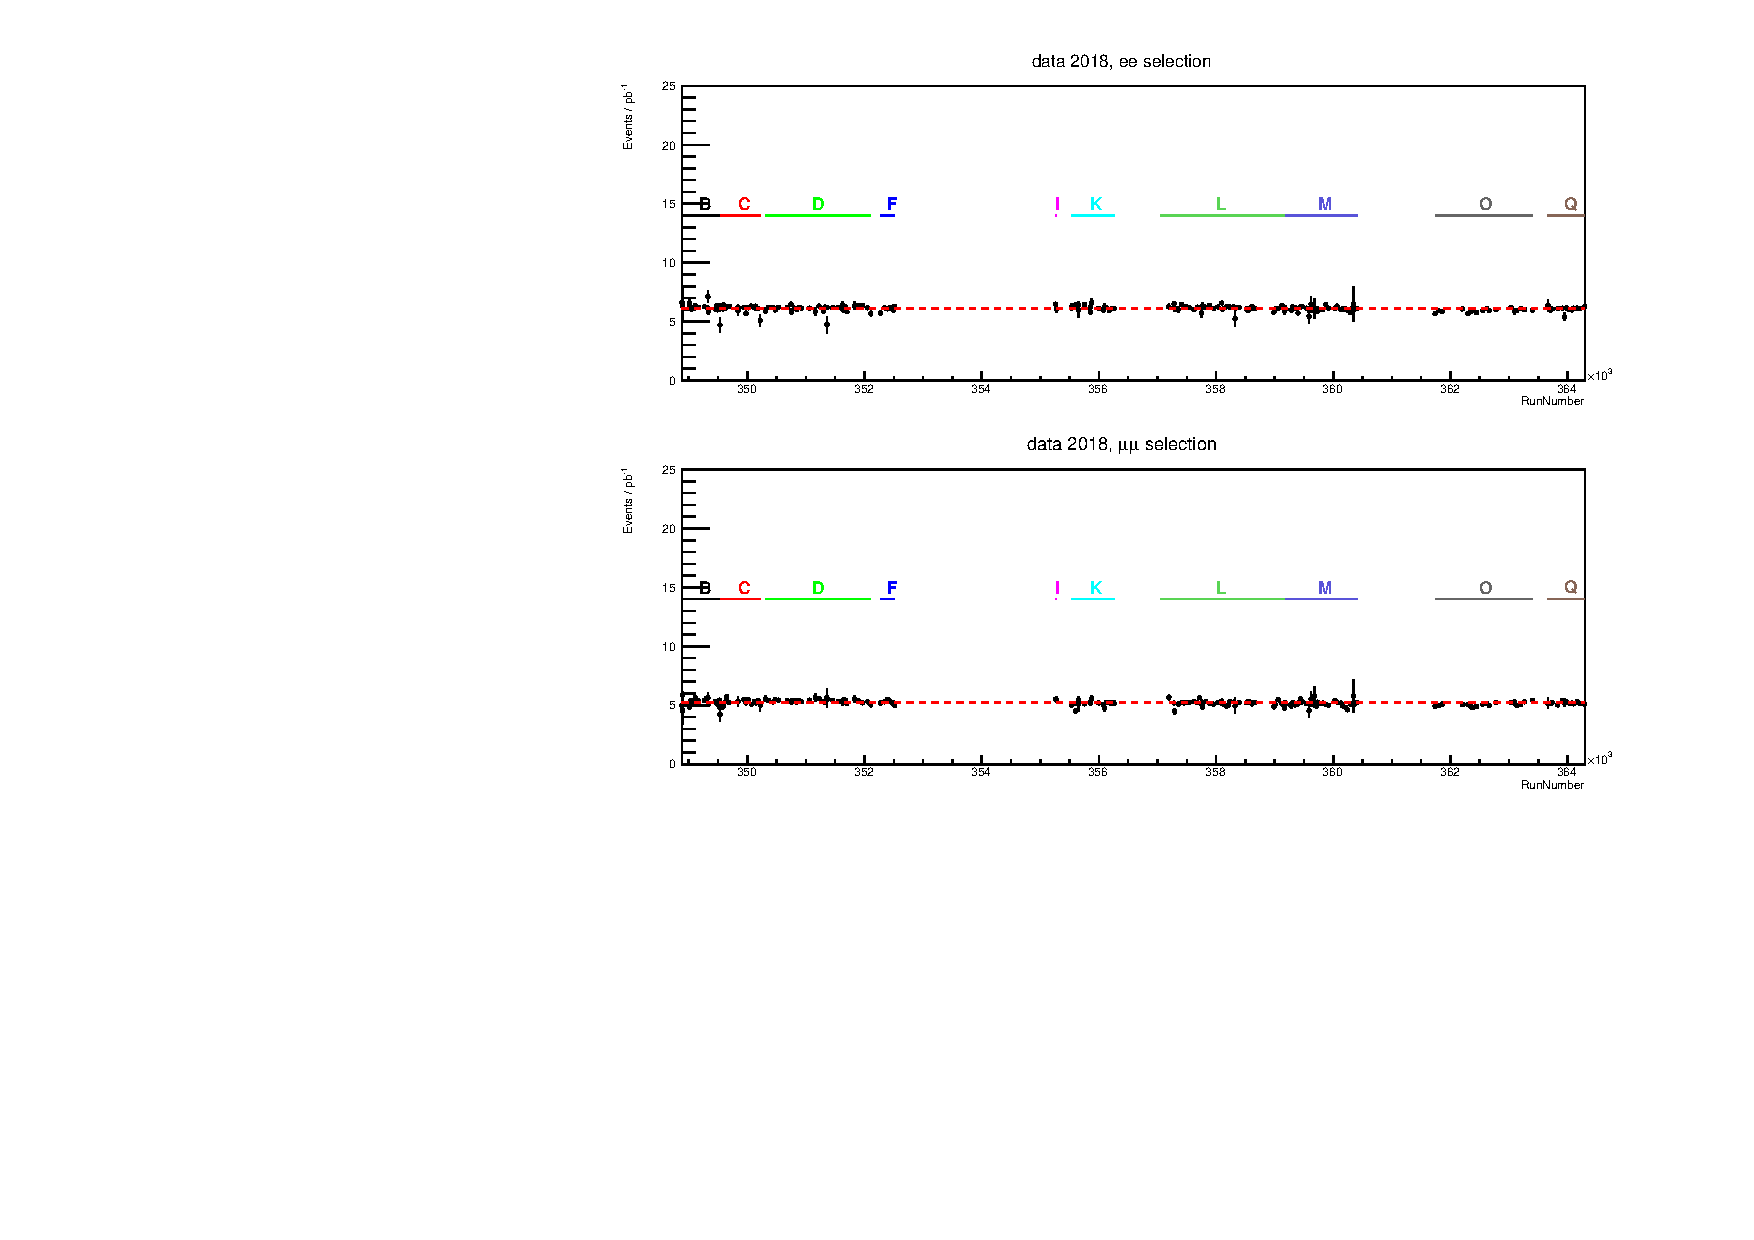
\includegraphics[width=\textwidth]{figures/analysis/datamc/Yields/compare_data_yields2018.pdf}
\caption{Data yields for the 2018 run period for the inclusive $ee$ (above) and $\mu\mu$ (below) selections Each letter on the legend correspond to the different data taking periods within a year~\cite{Aad:2019fac}.}
\label{fig:yields2018}
\end{figure}

\clearpage

\section{Monte Carlo samples}\label{sec:datamc:mc}
While the analysis is carried out in a data driven way, simulated samples for the background and signal are used to determine the appropriate functional form to fit the data, study background compositions, estimate uncertainties and evaluate signal. This section outlines the MC samples used for the background and signal samples.

While generators are available to produce events using higher order matrix elements are now available, it is often required to enhance the description of the process beyond the order of the generator used. Higher order QCD and EW corrections can modify the shape of the invariant mass distributions. Mass-dependent \emph{K}-factors can be derived taking the ratio of the higher order differential cross-section calculation over the available sample, e.g. next-to-next-to-leading order(NNLO) over the next-to-leading order (NLO). The \emph{K}-factors can then be applied to the invariant mass distribution on an event by event basis to produce higher order samples. 

\subsection{Background samples}\label{sec:datamc:mc:bkg}
The main backgrounds in decreasing order of importance are Drell-Yan (DY), top-quark ($t\bar{t}$), single-top-quark and diboson production. For the electron channel is it prohibitive to produce MC with enough events to accurately represent the expected QCD multijet distribution, due to the very small probabilities of jets faking electrons which pass the analysis selection. Therefore, the QCD and W+Jets processes in the dielectron channel are estimated with a data driven method~\cite{EXOT-2016-05}. For the muon channel the multijet background was studied and found to be negligible~\cite{EXOT-2016-05}, therefore, the contribution is neglected. 

The SM Drell-Yan process is modelled using the NLO \POWHEGBOX~\cite{Alioli:2010xd,Frixione:2007vw} event generator using the CT10~\cite{ct10} PDF together with \PYTHIAV{v8.186}~\cite{pythia8} is used for event showering. The DY samples are generated in slices of dilepton invariant mass, where 19 mass-binned samples were created with dilepton invariant mass ranging from \SI{120}{\giga\electronvolt} and $>$ \SI{5000}{\giga\electronvolt}, to increase the statistics of the samples in the high-mass regions. Corrections are applied to the DY samples to correct them from NLO to NNLO using using a mass dependent \emph{K}-factor is calculated with {\textsc{VRAP}} v0.9~\cite{vrap} and the CT14 NNLO PDF set~\cite{CT14} for QCD effects. {\textsc{MCSANC}}~\cite{MCSANC} is used for quantum electrodynamic corrections.  The diboson processes ($WW$, $WZ$ and $ZZ$) are generated at NLO using \SHERPA 2.1.1~\cite{Gleisberg:2008ta} with the CT10 PDF. Similar to the DY samples, the diboson samples were generated in invariant mass slices to increase the statistics of the sample. The $t\bar{t}$ background is generated at NLO using \POWHEGBOX with the NNPDF3.0NLO~\cite{Ball:2014uwa} PDF. Single top (s/t-channel) uses \POWHEGBOX with NNPDF3.0NLO PDF. A top quark mass of \SI{175.2}{\giga\electronvolt} is set for the generation of these samples. The top quark samples are normalised to the cross section at NNLO in QCD including resummation of the NNLO leading order soft gluon terms as provided by \textsc{Top++}2.0~\cite{Czakon:2011xx}.

The MC event generators for the hard-scattering process, showering and PDFs are listed in \cref{tab:MC}. A detailed description of the event simulation procedure is given in \cref{sec:simulation}. "Afterburner" generators such as \textsc{Photos}~\cite{Golonka:2005pn} for the final-state photon radiation (FSR) modelling, \textsc{MadSpin}~\cite{Artoisenet:2012st} to preserve top-quark spin correlations, and \textsc{EvtGen}~\cite{Lange:2001uf}, used for the modelling of $c$- and $b$-hadron decays, are also included in the simulation.

\begin{table}[htbp]
\centering
\tablesize{
\begin{tabular}{llp{5cm}}
\toprule
Background Process & ME Generator and ME PDFs & PS and non-perturbative effect with PDFs \\\hline
NLO Drell--Yan & \POWHEGBOX~\cite{Alioli:2010xd,Frixione:2007vw}, CT10~\cite{ct10}, \textsc{Photos} & \PYTHIAV{v8.186}~\cite{pythia8}, CTEQ6L1~\cite{ATL-PHYS-PUB-2014-021,Stump:2003yu}, \newline \textsc{EvtGen1.2.0} \\
$t\bar{t}$  & \POWHEGBOX, NNPDF3.0NLO~\cite{Ball:2014uwa} & \PYTHIAV{v8.230}, NNPDF23LO~\cite{Ball:2012cx}, \newline \textsc{EvtGen1.6.0} \\
Single top $s$-channel, $Wt$& \POWHEGBOX, NNPDF3.0NLO & \PYTHIAV{v8.230}, NNPDF23LO, \newline \textsc{EvtGen1.6.0} \\
Single top $t$-channel & \POWHEGBOX, NNPDF3.04fNLO, \textsc{MadSpin} & \PYTHIAV{v8.230}, NNPDF23LO,\newline  \textsc{EvtGen1.6.0}  \\
Diboson ($WW$, $WZ$ and $ZZ$) & \SHERPA 2.1.1~\cite{Gleisberg:2008ta}, CT10 &\SHERPA 2.1.1, CT10  \\\hline
Signal Process & & \\\hline
LO Drell--Yan & \PYTHIAV{v8.186}, NNPDF23LO  &  \PYTHIAV{v8.186}, NNPDF23LO, \newline \textsc{EvtGen1.2.0} \\
LO CI & \PYTHIAV{v8.186}, NNPDF23LO  &  \PYTHIAV{v8.186}, NNPDF23LO, \newline \textsc{EvtGen1.2.0} \\
\bottomrule
\end{tabular}
}
\caption[The event generators used for PDFs and generating matrix element (ME) and parton shower (PS) simulation of the signal and background processes.]{The event generators used for PDFs and generating matrix element (ME) and parton shower (PS) simulation of the signal and background processes. The top-quark mass is set to \SI{175.2}{\giga\electronvolt}.}
\label{tab:MC}
\end{table}

\subsection{Signal samples}\label{sec:datamc:mc:sig}
The \PYTHIAV{v8.230} generator is used to produce CI signal samples at leading-order (LO) using the NNPDF23LO PDF. Five benchmark values of $\Lambda$ from 10-\SI{30}{\tera\electronvolt} in steps of \SI{5}{\tera\electronvolt} were generated for each of the CI models. The CI shapes contain both the SM DY background and the interference between the DY and CI. 

It is possible to reweight the SM background to BSM signals when both the signal and background have the same initial and final states, due to  SM background particles being required as inputs for BSM signal+background differential cross sections. Therefore, an event dependent reweighting factor can be derived by taking the ratio of the SM and BSM (e.g CI) differential cross sections on an event by event basis. The reweighting scale factor is given by~\cite{EXOT-2016-05}:
\begin{equation}
    S = \frac{\frac{d\sigma}{d\hat{t}}(q\bar{q} \rightarrow \gamma, CI \rightarrow f\bar{f})}{\frac{d\sigma}{d\hat{t}}(q\bar{q} \rightarrow \gamma, Z \rightarrow f\bar{f})},
\end{equation}
where the numerator refers the BSM differential cross section and the denominator refers to the SM process only. It is possible to reweight any SM kinematic quantities to the correspond BSM one using this method as the differential cross sections are functions of event kinematics. This technique circumvents the requirement to generate MC samples for each potential signal hypothesis that needs to be tested, but, rather allowing for samples to be generated for any model by reweighting from a single background sample. 

Leading-order (LO) DY samples generated using \PYTHIAV{v8.186} with NNPDF23LO PDF is used in the reweighting procedure. The weights are applied to the LO DY events to transform into CI signal shapes, in steps of \SI{2}{\tera\electronvolt} between $\Lambda = \SI{12}{\tera\electronvolt}$ and $\Lambda = \SI{100}{\tera\electronvolt}$. In addition, dilepton mass dependent higher-order QCD and electroweak production corrections for signals are computed with the same methodology as for the DY background. While higher order QCD corrections are expected to be the same for signals and background, it is not clear the electroweak corrections can be treated the same. The addition of the electroweak corrections may be less conservative, however, it is deemed to be closer to the theoretically correct treatment than being over conservative and not including the corrections. 

\section{Transfer functions}\label{sec:datamc:transfer}
